
\documentclass{article}

\usepackage{polyglossia}
	\setmainlanguage{english}
\usepackage{amsmath}
\usepackage{siunitx}
\usepackage[margin=4cm]{geometry}
\usepackage{booktabs}
\usepackage{subcaption}
\usepackage{graphicx}
\usepackage{float}
\usepackage{amssymb}
\usepackage{xcolor}
\usepackage{listings}
    \lstset{language=Python,
	basicstyle=\footnotesize\ttfamily,
	breaklines=true,
	framextopmargin=50pt,
	frame=bottomline,
	backgroundcolor=\color{white!85!black},
	commentstyle=\color{blue},
	keywordstyle=\color{red},
	stringstyle=\color{orange!80!black}}
\usepackage{tikz}

\title{Computational Physics - Exercise 2}
\author{Maurice Donner u. Lukas Häffner}

\begin{document}

\maketitle
\newpage

\section*{1 - 4th Order Runge Kutta Method}

We compare the algorithms solution for different stepsizes h:

\begin{figure}[ht]
    \centering
    \begin{subfigure}{.32\textwidth}
	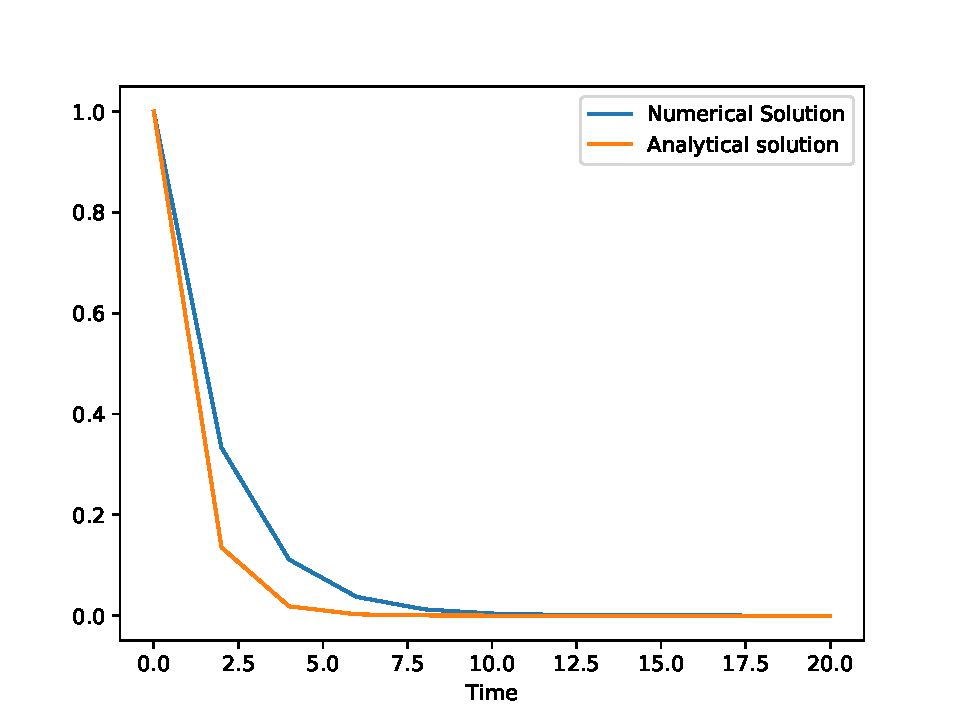
\includegraphics[width=\textwidth]{1_h_eq_2.pdf} 
	\caption{$h = 2$} 	
    \end{subfigure}
    \begin{subfigure}{.32\textwidth}
	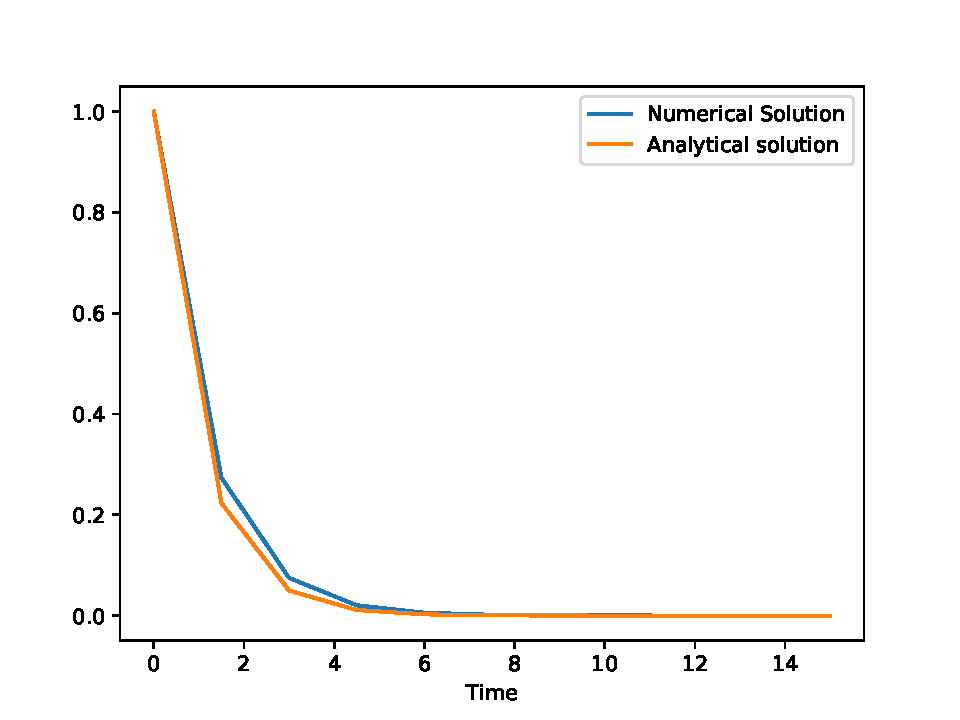
\includegraphics[width=\textwidth]{1_h_eq_1p5.pdf} 
	\caption{$h = 1.5$} 	
    \end{subfigure}
    \begin{subfigure}{.32\textwidth}
	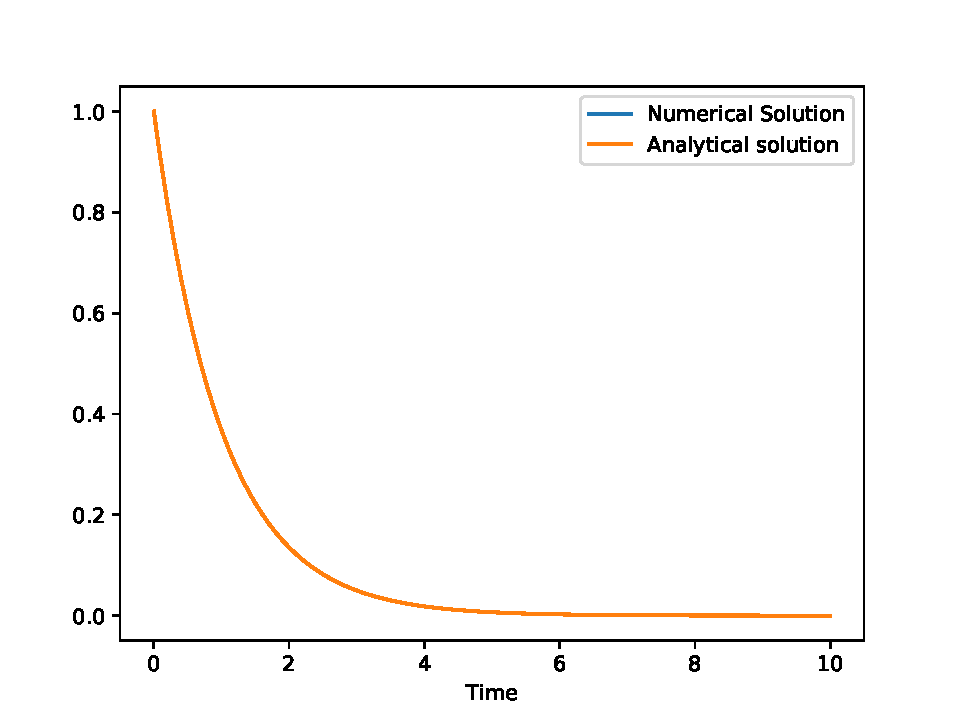
\includegraphics[width=\textwidth]{1_h_eq_0p1.pdf} 
	\caption{$h = 0.1$} 	
    \end{subfigure}
\end{figure}

The Numerical approximation seems to converge really quickly towards the
analytical solution, even for relatively large stepsizes \( h \).

\section*{2 - Three-Body Problem}

In order to integrate the Tree-Body Problem a lot of startparameters have to
be given to the system.
\begin{align*}
    G &= m_1 = m_2 = m_3 = 1 \\
    (y_1,y_2) & = −0.97000436 , 0.24308753 \\
    (y_3,y_4) & = −0.46620368 , -0.43236573 \\
    (y_5,y_6) & = 0.97000436 , -0.24308753 \\
    (y_7,y_8) & = −0.46620368 , -0.43236573 \\
    (y_9,y_{10}) & = 0 , 0 \\
    (y_{11},y_{12}) & = 0.93240737 , 0.86473146 \\
\end{align*}

The indices of the different starting values are as follows

\begin{align*}
(y_1,y_5,y_9) &: \ \text{x-Coordinate of Particles} \\
(y_2,y_6,y_{10}) &: \ \text{y-Coordinate of Particles} \\
(y_3,y_7,y_{11}) &: v_x \ \text{Initial Velocity of particles in x-Direction} \\
(y_4,y_8,y_{12}) &: v_y \ \text{Initial Velocity of particles in y-Direction} \\
\end{align*}

We store our information of the differential equations in a function
\texttt{function(y0,x0,m)}. Into this function we feed our \( 4n \)-Dimensional
vector y, that contains all the information of our n masses as described above.

The first differential equation we input is simply 
\( f(x_i,y_i) = ( v_{x_i} , v_{y_i} ) \):
\begin{lstlisting}
def function(y0,x0,m): # This calculates ALL derivatives
    out = np.zeros(y.shape) # y.shape = (12,)
    for index in np.arange(0,len(y0),4): # iterate over the 3 Masses
            out[index] = y0[index+2] # f(x) = vx
            out[index+1] = y0[index+3] # f(y) = vy
    return out
\end{lstlisting}
What's missing yet is the second differential equation. For that we need to sum
over all the forces resulting from other masses in the system. For that we will
create a second index, and calculate just those forces, where \( i \ne j \).
For \( \dot{v}_{x_i} \) for example, we get:
\[ 
    f(v _{x_i}) = v _{x_i} + G \cdot m_j \cdot \frac{x_j - x_i}{((x_j - x_i)^2
    + (y_j-y_i)^2)^{3/2}} = v _{x_i} + G \cdot m_j \cdot \frac{r_x}{|r|^3}
\]
Adding this to our \texttt{for}-loop, we get:
\begin{lstlisting}
def function(y0,x0,m): # This calculates ALL derivatives
    out = np.zeros(y.shape) # y.shape = (12,)
    for index in np.arange(0,len(y0),4): # iterate over the 3 Masses
            out[index] = y0[index+2] # f(x) = vx
            out[index+1] = y0[index+3] # f(y) = vy
            for indexx in np.arange(0,len(y0),4):
                if (index != indexx): # sum dynamically over non-equal indizes 
                    out[index+2] += G*m[(int)(indexx/4)]*(y0[indexx]-y0[index]
                    )/((y0[indexx]-y0[index])**2+(y0[indexx+1]-y0[index+1]
                    )**2)**1.5 # f(vx) = vx+G*m*(r/|r|*3)

                    out[index+3] += G*m[(int)(indexx/4)]*(y0[indexx+1]-y0[index+1]
                    )/((y0[indexx]-y0[index])**2+(y0[indexx+1]-y0[index+1]
                    )**2)**1.5 # f(vy) = vy+G*m*(r/|r|*3)
    return out
\end{lstlisting}


Next we write a simple function that stores all of the information provided by
the rk4 method nicely, which makes for an easy plot:

\begin{lstlisting}
def final(h,n,init_vec,m):
    y0,x0 = init_vec
    y0,x0 = rk4(y0,x0,function,h,n,{"m" : m})

    out_x0 = np.zeros(x0.shape)
    out_y0 = np.zeros(x0.shape)
    out_x1 = np.zeros(x0.shape)
    out_y1 = np.zeros(x0.shape)
    out_x2 = np.zeros(x0.shape)
    out_y2 = np.zeros(x0.shape)

    for index, i in enumerate(y0):
        out_x0[index] = i[0]
        out_y0[index] = i[1]
        out_x1[index] = i[4]
        out_y1[index] = i[5]
        out_x2[index] = i[8]
        out_y2[index] = i[9]

    return ((out_x0, out_y0), (out_x1, out_y1), (out_x2, out_y2))
\end{lstlisting}

Playing around with different stepsizes and runtimes, we can easily get a
plot where all the individual particle trajectories are distinguishable.
For h = 0.1 and n = 200 we found:
\begin{figure}[ht]
    \centering
    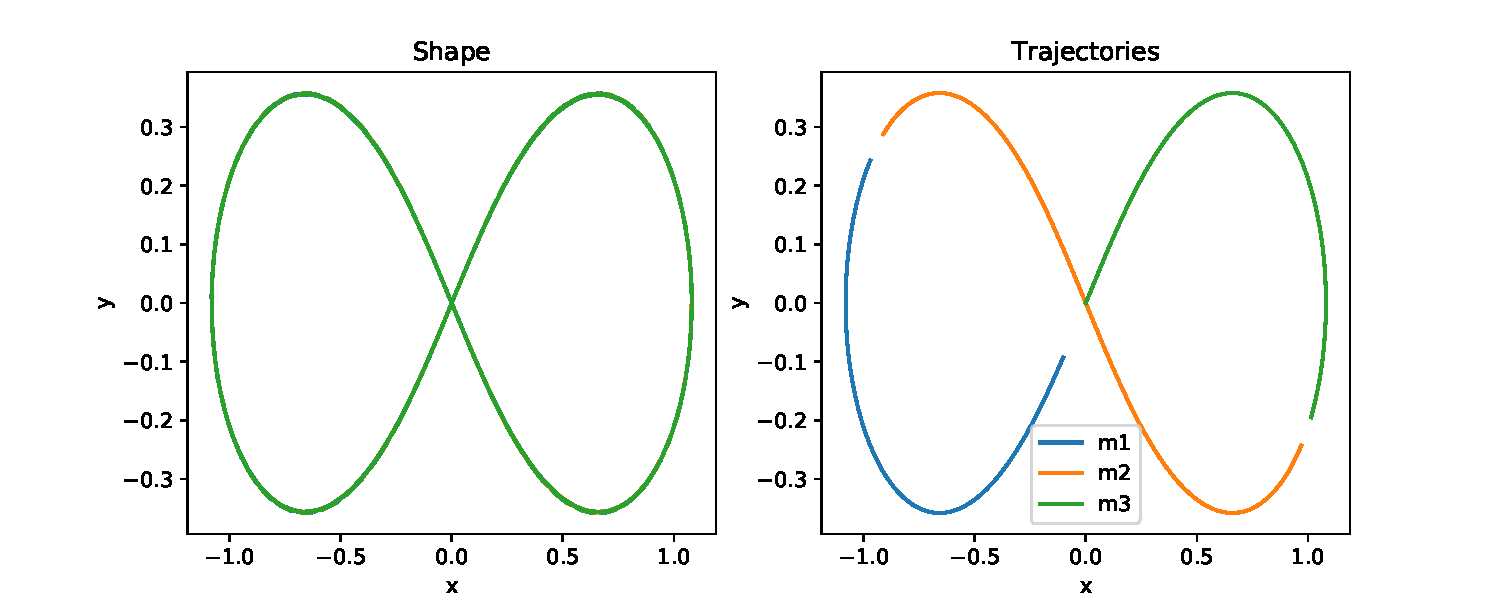
\includegraphics[width=\textwidth]{fig2a.pdf} 
    \caption{Stable Solution for the 3-Body-Problem}
\end{figure}
 
\newpage
\subsection*{b)}

Next, we will look at the Meissel-Burrau Problem for three Masses, with initial
velocity of 0:
\begin{figure}[ht]
    \centering
\begin{subfigure}{.2\textwidth}
    \begin{align*}
	m_1 &= 3 \\
	m_2 &= 4 \\
	m_3 &= 5
    \end{align*}
\end{subfigure}
\begin{subfigure}{.3\textwidth}
    \centering
\begin{tikzpicture}[scale=.7]
    \draw (0,0) -- (4,0) -- (0,3) -- (0,0);
    \draw (0,1.5) node [anchor=east] {$l_1 = 3$};
    \draw (2,0) node [anchor=north] {$l_2 = 4$};
    \draw (2.5,1.5) node [anchor=south] {$l_3 = 5$};
    \filldraw [blue!50!black] (0,0) circle [radius=2pt] node [anchor=east] {$m_3$};
    \filldraw [blue!50!black] (4,0) circle [radius=2pt] node [anchor=west] {$m_1$};
    \filldraw [blue!50!black] (0,3) circle [radius=2pt] node [anchor=east] {$m_2$};
    \draw (0.5,0) arc[start angle=0, end angle=90, radius=0.5];
    \filldraw [black] (0.2,0.2) circle [radius=1pt];
\end{tikzpicture}
\end{subfigure}
\caption{Meissel-Burrau Problem}
\end{figure}

We transform those coordinates into the CMS system, and run the program for
different stepsizes and computation times. We immediately see that choosing
smaller stepsizes yields much more accurate interactions between the Masses:
\begin{figure}[H]
    \centering
    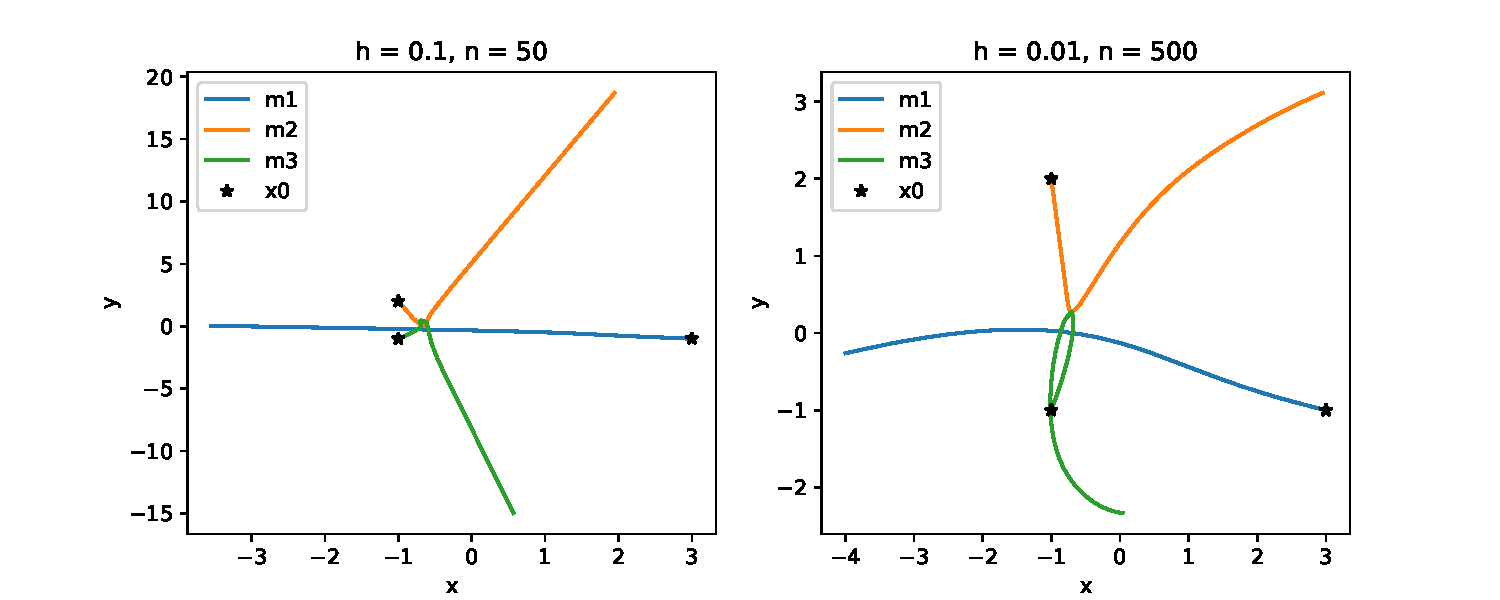
\includegraphics[width=\textwidth]{fig2b_large.pdf} 
    \caption{Meissel-Burrau Problem for different Stepsizes} 
    \label{fig:2b}
\end{figure}

Next, we add a little block extra code to our rk4-loop, that measures the
distances of each of the 3 masses. First we need a distance function:
\begin{lstlisting}
    def dist(r1,r2):
	return ((r2[0]-r1[0])**2+(r2[1]-r1[1])**2)**0.5
\end{lstlisting}
Next we use that to find the minimum distance between the masses, by storing
the current distance in a variable, and check with each step, if that variable
becomes smaller:

\begin{lstlisting}
def rk4(y0, x0, f, h, n, f_args = {}):
    yn = np.zeros((n+1, y0.shape[0]))
    xn = np.zeros(n+1)
    yn[0,:] = y0
    xn[0] = x0
    mindist12 = 5 # initial distance
    mindist23 = 3 # initial distance
    mindist31 = 4 # initial distance
    mint12 = 0
    mint23 = 0
    mint31 = 0
    
    for n in np.arange(1,n+1,1):
        yn[n,:], xn[n] = rk4_step(y0 = yn[n-1,:], x0 = xn[n-1], f = f, h = h, f_args = f_args)
        # Calculate distances of masses:
        r1 = np.array([yn[n,0],yn[n,1]])
        r2 = np.array([yn[n,4],yn[n,5]])
        r3 = np.array([yn[n,8],yn[n,9]])
        
        dist12 = dist(r1,r2)
        dist23 = dist(r2,r3)
        dist31 = dist(r3,r1)

        if (dist12 <= mindist12): # if minimum distance smaller than before, save
            mindist12 = dist12
            mint12 = n 
        if (dist23 <= mindist23):
            mindist23 = dist23
            mint23 = n 
        if (dist31 <= mindist31):
            mindist31 = dist31
            mint31 = n 

    print('Minimum distances for h = ', round(h,10), 'and n =', n)

    print('Minimum Distance of Masses 1 and 2: ',
            round(mindist12,2), 'at t =', mint12)
    print('Minimum Distance of Masses 2 and 3: ',
            round(mindist23,2), 'at t =', mint23)
    print('Minimum Distance of Masses 3 and 1: ',
            round(mindist31,2), 'at t =', mint31, '\n')

    return(yn, xn)
\end{lstlisting}

In the following table, we examine the minimum distances together with the time
at which they occur for different stepsizes h:
\begin{table}[H]
    \centering
    \begin{tabular}{lcc}
	h & Distance $|r|$ & Time $t$ \\
	\toprule 
	0.1 & $1 \leftrightarrow 2$ = 2.65 & 21 \\ 
	& $2 \leftrightarrow 3$ = 0.15 & 21 \\
	& $3 \leftrightarrow 1$ = 2.15 & 24 \\ \midrule
	0.01 & $1 \leftrightarrow 2$ = 2.20 & 270 \\ 
	& $2 \leftrightarrow 3$ = 0.03 & 188 \\
	& $3 \leftrightarrow 1$ = 1.76 & 310 \\ \midrule
	0.001 & $1 \leftrightarrow 2$ = 2.99 & 1902 \\ 
	& $2 \leftrightarrow 3$ = 0.01 & 1902 \\
	& $3 \leftrightarrow 1$ = 2.25 & 1964 \\ \midrule
	0.0001 & $1 \leftrightarrow 2$ = 1.77 & 29444 \\ 
	& $2 \leftrightarrow 3$ = 0.01 & 18793 \\
	& $3 \leftrightarrow 1$ = 0.54 & 30191 \\
\bottomrule 
\end{tabular}
\caption{Minimum mass distances at different stepsizes}
\end{table}

From this, we see the problem resulting out of this arrangement of masses.
At a certain t, which occurs usually at around \( 19 \cdot 0.1 \) steps, two
of the masses get really close, so that \( v \), in some cases, becomes very large. That
will result in \( m_2 \) and \( m_3 \) rapidly slingshotting each other out of
the system. This effect is most visible at \( h = 0.001 \), whereas at
\( h = 0.0001 \) we get a better result again:
\begin{figure}[ht]
    \centering
    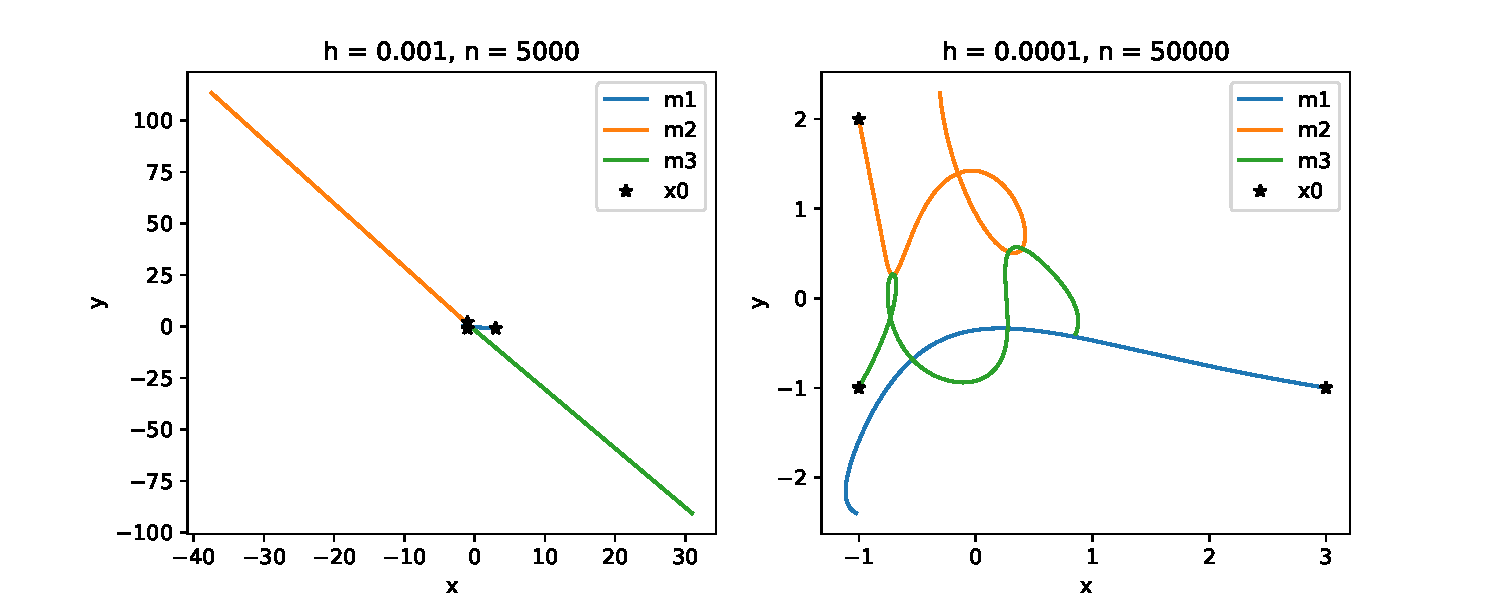
\includegraphics[width=\textwidth]{fig2b_small.pdf} 
    \caption{Particle trajectories for small stepsizes $h$} 
\end{figure}

Finally, we want to plot the particle distance and energy error as functions of
time. It is interesting to see, that the Energy error becomes more apparent while
approaching \( h=0.001 \) but then decreases for even smaller \( h \):
\begin{figure}[ht]
    \centering
    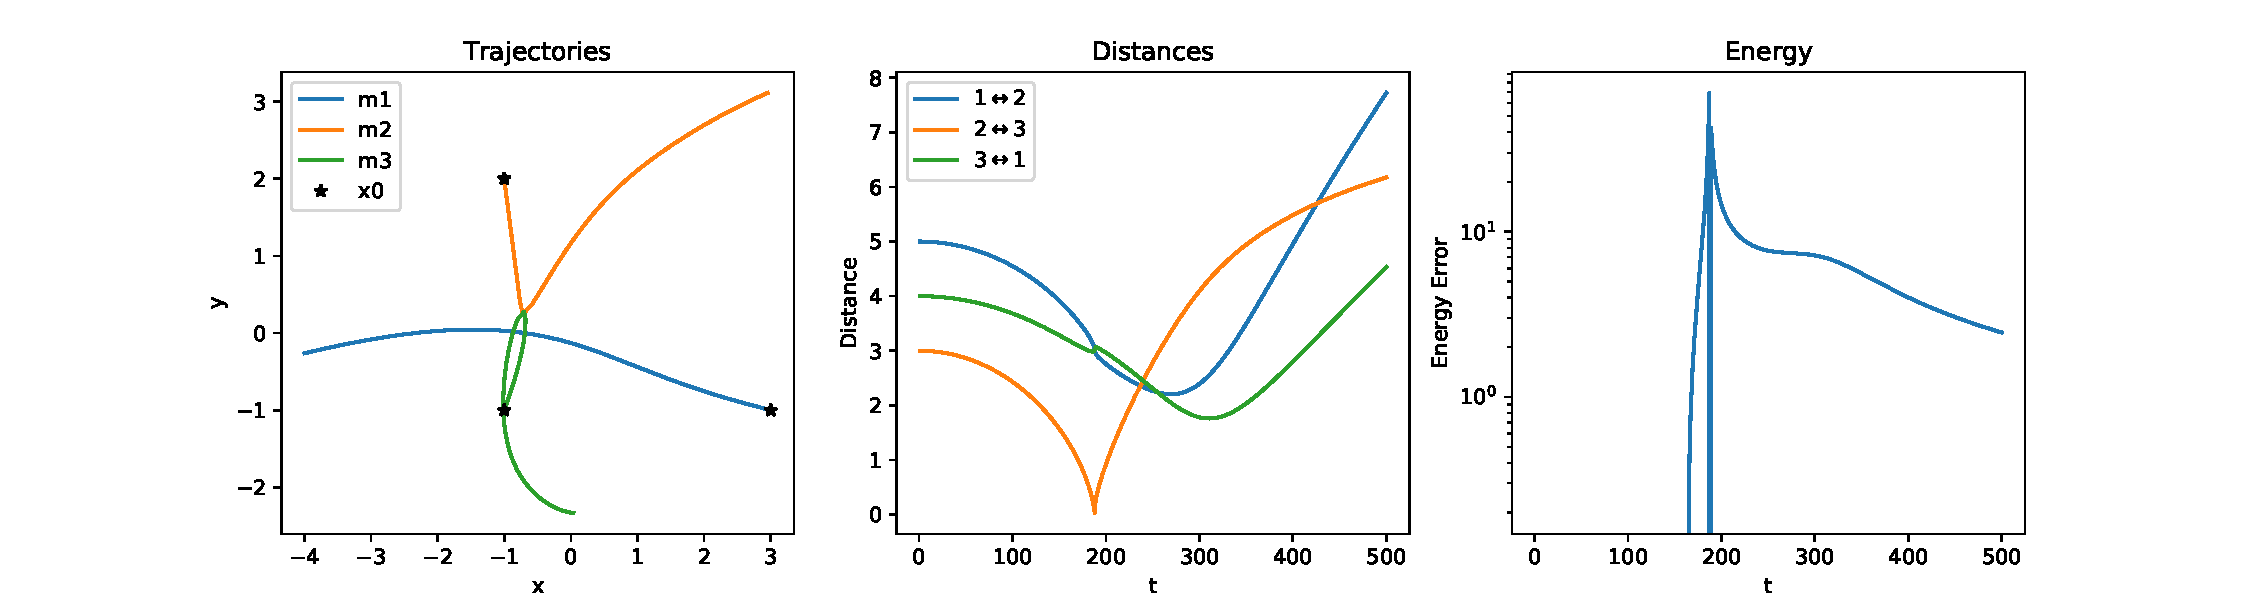
\includegraphics[width=\textwidth]{fig2b_distances_large.pdf} 
    \caption{Energy Error for $h = 0.01$ and $n = 500$}  
\end{figure}
\begin{figure}[ht]
    \centering
    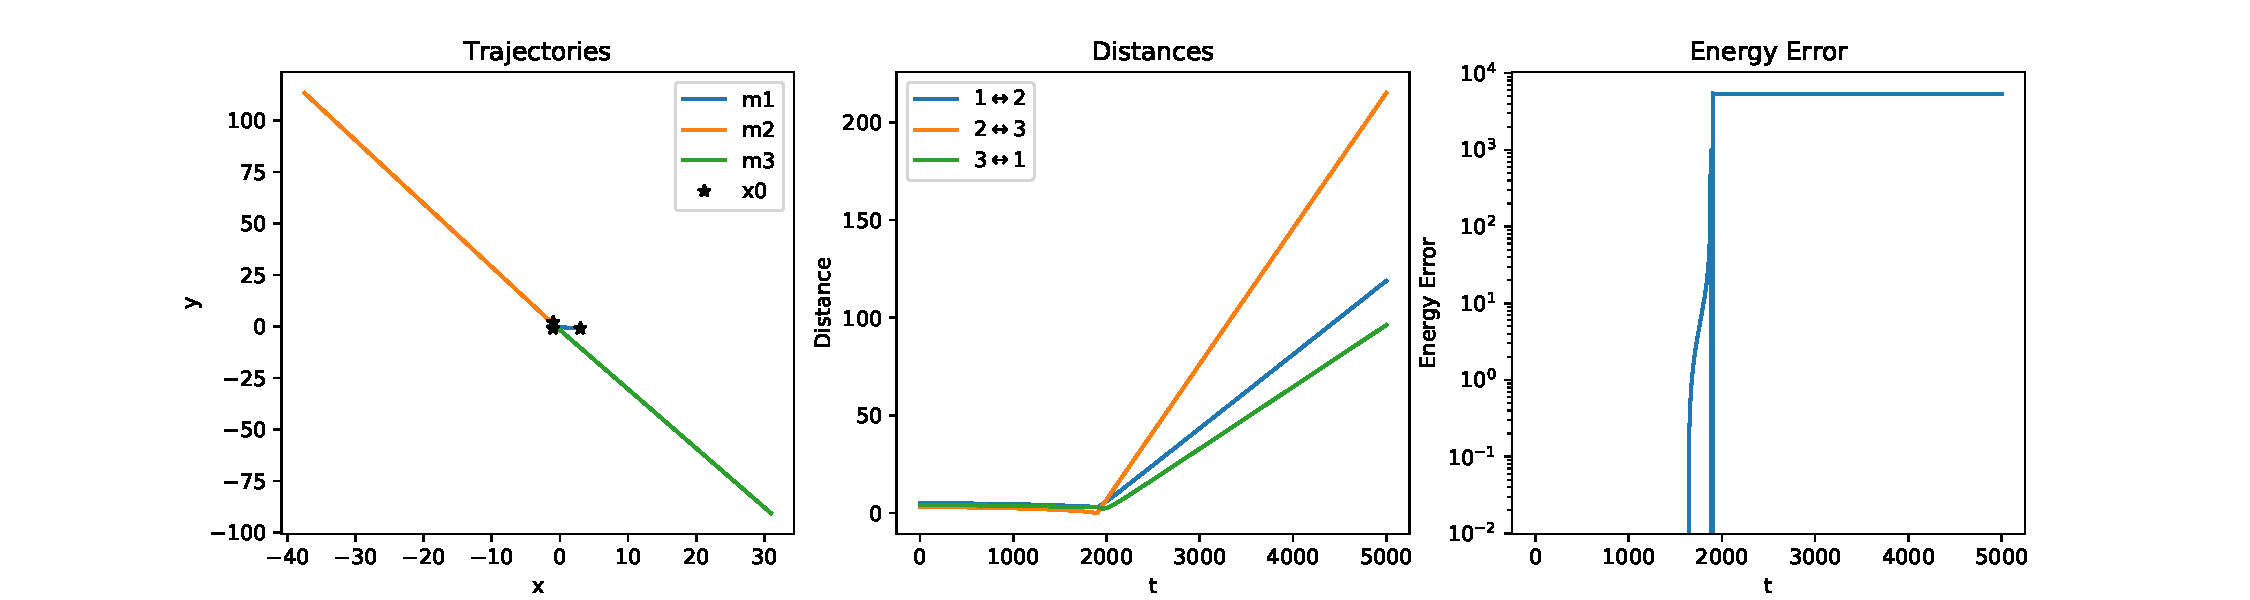
\includegraphics[width=\textwidth]{fig2b_distances_medium.pdf} 
    \caption{Energy Error for $h = 0.001$ and $n = 5000$}  
\end{figure}
\begin{figure}[ht]
    \centering
    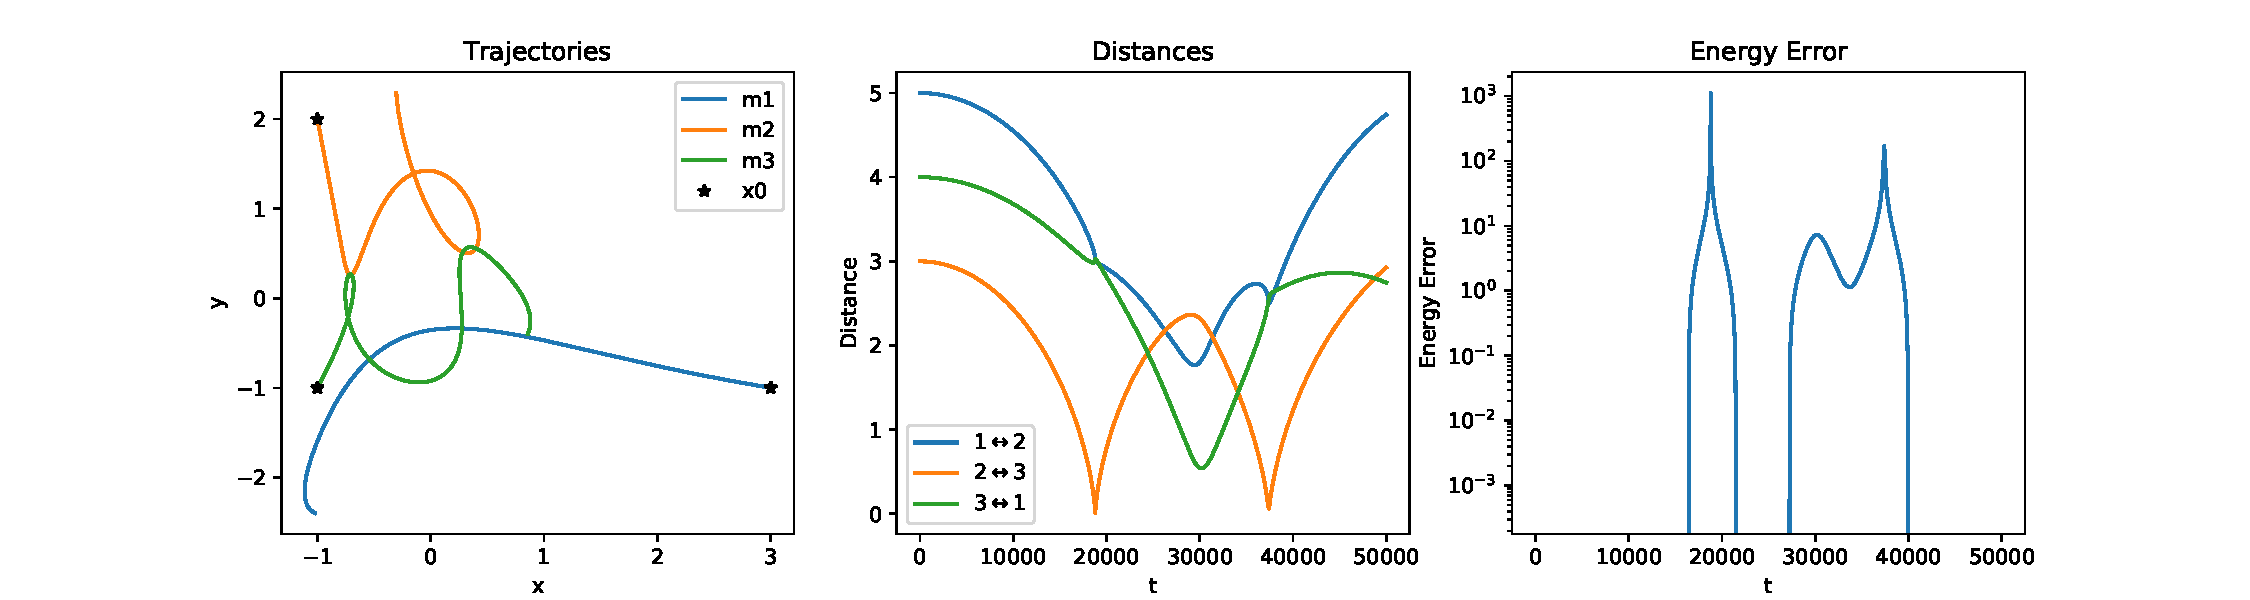
\includegraphics[width=\textwidth]{fig2b_distances_small.pdf} 
    \caption{Energy Error for $h = 0.0001$ and $n = 50000$}  
\end{figure}

\end{document}

